%  template.tex for Biometrics papers
%
%  This file provides a template for Biometrics authors.  Use this
%  template as the starting point for creating your manuscript document.
%  See the file biomsample.tex for an example of a full-blown manuscript.

%  ALWAYS USE THE referee OPTION WITH PAPERS SUBMITTED TO BIOMETRICS!!!
%  You can see what your paper would look like typeset by removing
%  the referee option.  Because the typeset version will be in two
%  columns, however, some of your equations may be too long. DO NOT
%  use the \longequation option discussed in the user guide!!!  This option
%  is reserved ONLY for equations that are impossible to split across 
%  multiple lines; e.g., a very wide matrix.  Instead, type your equations 
%  so that they stay in one column and are split across several lines, 
%  as are almost all equations in the journal.  Use a recent version of the
%  journal as a guide. 
%  
\documentclass[useAMS,referee]{biom}

%documentclass[useAMS]{biom}
%
%  If your system does not have the AMS fonts version 2.0 installed, then
%  remove the useAMS option.
%
%  useAMS allows you to obtain upright Greek characters.
%  e.g. \umu, \upi etc.  See the section on "Upright Greek characters" in
%  this guide for further information.
%
%  If you are using AMS 2.0 fonts, bold math letters/symbols are available
%  at a larger range of sizes for NFSS release 1 and 2 (using \boldmath or
%  preferably \bmath).
% 
%  Other options are described in the user guide. Here are a few:
% 
%  -  If you use Patrick Daly's natbib  to cross-reference your 
%     bibliography entries, use the usenatbib option
%  -  If you use \includegraphics (graphicx package) for importing graphics
%     into your figures, use the usegraphicx option
% 
%  If you wish to typeset the paper in Times font (if you do not have the
%  PostScript Type 1 Computer Modern fonts you will need to do this to get
%  smoother fonts in a PDF file) then uncomment the next line
%  \usepackage{Times}

%%%%% PLACE YOUR OWN MACROS HERE %%%%%

\def\bSig\mathbf{\Sigma}
\newcommand{\VS}{V\&S}
\newcommand{\tr}{\mbox{tr}}

%  The rotating package allows you to have tables displayed in landscape
%  mode.  The rotating package is NOT included in this distribution, but
%  can be obtained from the CTAN archive.  USE OF LANDSCAPE TABLES IS
%  STRONGLY DISCOURAGED -- create landscape tables only as a last resort if
%  you see no other way to display the information.  If you do do this,
%  then you need the following command.

%\usepackage[figuresright]{rotating}

%%%%%%%%%%%%%%%%%%%%%%%%%%%%%%%%%%%%%%%%%%%%%%%%%%%%%%%%%%%%%%%%%%%%%

%  Here, place your title and author information.  Note that in 
%  use of the \author command, you create your own footnotes.  Follow
%  the examples below in creating your author and affiliation information.
%  Also consult a recent issue of the journal for examples of formatting.

\title[Visualization methods for RNA-sequencing data]{Visualization methods for RNA-sequencing data}

%  Here are examples of different configurations of author/affiliation
%  displays.  According to the Biometrics style, in some instances,
%  the convention is to have superscript *, **, etc footnotes to indicate 
%  which of multiple email addresses belong to which author.  In this case,
%  use the \email{ } command to produce the emails in the display.

%  In other cases, such as a single author or two authors from 
%  different institutions, there should be no footnoting.  Here, use
%  the \emailx{ } command instead. 

%  The examples below corrspond to almost every possible configuration
%  of authors and may be used as a guide.  For other configurations, consult
%  a recent issue of the the journal.

%  Single author -- USE \emailx{ } here so that no asterisk footnoting
%  for the email address will be produced.

%\author{John Author\emailx{email@address.edu} \\
%Department of Statistics, University of Warwick, Coventry CV4 7AL, U.K.}

%  Two authors from the same institution, with both emails -- use
%  \email{ } here to produce the asterisk footnoting for each email address

%\author{John Author$^{*}$\email{author@address.edu} and
%Kathy Authoress$^{**}$\email{email2@address.edu} \\
%Department of Statistics, University of Warwick, Coventry CV4 7AL, U.K.}

%  Exactly two authors from different institutions, with both emails  
%  USE \emailx{ } here so that no asterisk footnoting for the email address
%  is produced.

%  Three or more authors from same institution with all emails displayed
%  and footnoted using asterisks -- use \email{ } 

%\author{John Author$^*$\email{author@address.edu}, 
%Jane Author$^{**}$\email{jane@address.edu}, and 
%Dick Author$^{***}$\email{dick@address.edu} \\
%Department of Statistics, University of Warwick, Coventry CV4 7AL, U.K}

%  Three or more authors from same institution with one corresponding email
%  displayed

%\author{John Author$^*$\email{author@address.edu}, 
%Jane Author, and Dick Author \\
%Department of Statistics, University of Warwick, Coventry CV4 7AL, U.K}

%  Three or more authors, with at least two different institutions,
%  more than one email displayed 

%\author{John Author$^{1,*}$\email{author@address.edu}, 
%Kathy Author$^{2,**}$\email{anotherauthor@address.edu}, and 
%Wilma Flinstone$^{3,***}$\email{wilma@bedrock.edu} \\
%$^{1}$Department of Statistics, University of Warwick, Coventry CV4 7AL, U.K \\
%$^{2}$Department of Biostatistics, University of North Carolina at 
%Chapel Hill, Chapel Hill, North Carolina, U.S.A. \\
%$^{3}$Department of Geology, University of Bedrock, Bedrock, Kansas, U.S.A.}

%  Three or more authors with at least two different institutions and only
%  one email displayed

%\author{John Author$^{1,*}$\email{author@address.edu}, 
%Wilma Flinstone$^{2}$, and Barney Rubble$^{2}$ \\
%$^{1}$Department of Statistics, University of Warwick, Coventry CV4 7AL, U.K \\
%$^{2}$Department of Geology, University of Bedrock, Bedrock, Kansas, U.S.A.}

\usepackage{graphicx}
\begin{document}


%  This will produce the submission and review information that appears
%  right after the reference section.  Of course, it will be unknown when
%  you submit your paper, so you can either leave this out or put in 
%  sample dates (these will have no effect on the fate of your paper in the
%  review process!)

%  These options will count the number of pages and provide volume
%  and date information in the upper left hand corner of the top of the 
%  first page as in published papers.  The \pagerange command will only
%  work if you place the command \label{firstpage} near the beginning
%  of the document and \label{lastpage} at the end of the document, as we
%  have done in this template.

%  Again, putting a volume number and date is for your own amusement and
%  has no bearing on what actually happens to your paper!  

%  The \doi command is where the DOI for your paper would be placed should it
%  be published.  Again, if you make one up and stick it here, it means 
%  nothing!

%  This label and the label ``lastpage'' are used by the \pagerange
%  command above to give the page range for the article.  You may have 
%  to process the document twice to get this to match up with what you 
%  expect.  When using the referee option, this will not count the pages
%  with tables and figures.  

\label{firstpage}

%  put the summary for your paper here

\begin{abstract}
This is the summary for this paper.
\end{abstract}

%  Please place your key words in alphabetical order, separated
%  by semicolons, with the first letter of the first word capitalized,
%  and a period at the end of the list.
%

\begin{keywords}
Data visualization; Exploratory data analysis; Interactive graphics; RNA-sequencing; Statistical graphics
\end{keywords}

%  As usual, the \maketitle command creates the title and author/affiliations
%  display 

\maketitle

%  If you are using the referee option, a new page, numbered page 1, will
%  start after the summary and keywords.  The page numbers thus count the
%  number of pages of your manuscript in the preferred submission style.
%  Remember, ``Normally, regular papers exceeding 25 pages and Reader Reaction 
%  papers exceeding 12 pages in (the preferred style) will be returned to 
%  the authors without review. The page limit includes acknowledgements, 
%  references, and appendices, but not tables and figures. The page count does 
%  not include the title page and abstract. A maximum of six (6) tables or 
%  figures combined is often required.''

%  You may now place the substance of your manuscript here.  Please use
%  the \section, \subsection, etc commands as described in the user guide.
%  Please use \label and \ref commands to cross-reference sections, equations,
%  tables, figures, etc.
%
%  Please DO NOT attempt to reformat the style of equation numbering!
%  For that matter, please do not attempt to redefine anything!

\section{Introduction}
\label{s:Introduction}

RNA-sequencing (RNA-seq) uses next-generation sequencing (NGS) to estimate the quantity of RNA in biological samples at given timepoints. In recent years, decreasing cost and increasing throughput has rendered RNA-seq an attractive alternative to transcriptome profiling. Prior to RNA-seq, gene expression studies were performed with microarray techniques, which required prior knowledge of reference sequences. RNA-seq does not have this limitation, and has enabled a new range of applications such as transcriptome de novo assembly (Grabherr et al., 2011; Robertson et al., 2010) and detection of alternative splicing processes (Anders, Reyes, and Huber, 2012; Pan et al., 2008). Coupled with its high resolution and sensitivity, RNA-seq will likely revolutionize our understanding of the intricacies of eukaryotic transcriptomes (Wang, Gerstein, and Snyder, 2009; Zhao et al., 2014).

Gene expression data is multivariate data, and its basic form is a matrix containing mapped read counts for \textit{n} rows of genes and \textit{p} columns of samples. These mapped read counts provide estimations of the gene expression levels across samples. Researchers typically conduct RNA-seq studies to identify differentially expressed genes (DEGs) between treatment groups. In most popular RNA-seq analysis packages, this objective is approached with models, such as the negative binomial model (Anders and Huber, 2010; Trapnell et al., 2013; Trapnell et al., 2012; Robinson et al., 2010) and linear regression models (Law et al., 2014).

Initially, it was widely claimed that RNA-seq produced unbiased data that did not require sophisticated normalization (Wang et al., 2009; Morin et al., 2008; Marioni et al., 2008). However, numerous studies have since revealed that RNA-seq data is replete with biases and that accurate detection of DEGs is not a negligible task. Problems that complicate the analysis of RNA-seq data include nucleotide-specific and read-position specific biases (Hansen et al., 2010), biases related to gene lengths and sequencing depths (Oshlack, Robinson, and Young, 2010; Robinson and Oshlack, 2010), biases introduced during library preparation (McIntyre et al., 2011), biases pertaining to the number of replications (Schurch et al., 2016), biases derived from overlapping senseantisense transcripts and gene isoforms (Trapnell et al., 2013), and the confounding combination of technical and biological variability (Bullard et al., 2010).

In light of these complications, researchers should analyze RNA-seq data like they would any other biased multivariate data. Simply applying models to such data is problematic because models have assumptions that they alone cannot call into question. Fortunately, data visualization enables researchers to see patterns and problems they may not otherwise detect with traditional modeling. As a result, the most effective approach to analyze data is to iterate between models and visuals, and to enhance the appropriateness of applied models based on feedback from visuals (Unwin, 1992; Shneiderman, 2002).

When visualizing RNA-seq data, we primarily want to compare the variability between replicates and between treatment groups. This is best achieved by viewing the mapped read count distributions across all genes and samples. Unfortunately, the few visual tools available in popular RNA-seq packages do not allow users to effectively view their data in this manner.

Here, we use real RNA-seq data to demonstrate that our visualization tools can detect normalization problems, DEG designation problems, and common errors in the analysis pipeline. We also show that our tools can identify genes of interest that cannot otherwise be obtained by any models. In line with modern multivariate data exploration, we emphasize that interactive graphics should be an indisposable component of RNA-seq analysis. Researchers should be able to quickly flip through plots of genes that appear promising or problematic, and link between different types of plots to quickly obtain various perspectives of their data. In this paper, we are not proposing that users completely change their approach to RNA-seq analysis. Instead, we propose that users simply modify their approach to RNA-seq analysis by assessing the sensibility of their models with multivariate graphical tools, namely parallel coordinate plots, scatterplot matrices, and replicate line plots.

\section{Parallel Coordinate Plots}
\label{s:Parallel Coordinate Plots}

Parallel coordinate plots are essential to visually verify the relationships between variables in multivariate data. A parallel coordinate plot draws each row (gene) in the data table as a line. Connections between samples with positive correlations will be flat, and connections between samples with negative correlations will be crossed. The ideal dataset will have large variability between treatment groups but little variability between replicates. Researchers can quickly confirm this with a parallel coordinate plot: There should be flat connections between replicates but crossed connections between treatment groups.

There are several packages within the BioConductor software that provide graphics for RNA-seq data analysis (Huber et al., 2015). Two of the most common graphic techniques are side-by-side boxplots and Multidimensional Scaling (MDS) plots (Love, Huber, and Anders, 2014; Risso et al., 2011; Robinson et al., 2010; Su et al., 2016; Ritchie et al., 2015; Marini, 2017). Unfortunately, these plots can hide problems that still exist in the data even after normalization and that could be better detected with parallel coordinate plots.

Figure~\ref{2group} exemplifies this problem for two simulated datasets, one displayed on the left half of the figure and the other displayed on the right half of the figure. Each dataset contains two treatment groups (A and B) with three replicate samples. We cannot detect any notable differences between the left and right datasets from the side-by-side boxlots at the top of the figure as they both show fairly consistent five number summaries across their six samples. Likewise, we cannot detect any notable differences between the datasets from the MDS plots in the middle of the figure as they both suggest that the datasets are clustered by the two treatment groups, although the first replicate from treatment group A appears as an outlier in the right MDS plot.

Despite this, we immediately see from the parallel coordinate plots at the bottom of the figure that the left and right datasests have an important difference. The left dataset has consistent (level) lines between replicates and inconsistent (crossed) lines between treatment groups. This suggests that some of the genes (lines) have consistently low values for treatment group A and consistently high values for treatment group B, while some genes have the opposite phenomenon. As a result, these plotted genes are likely candidates for differential expression. In contrast, the right dataset does not possess this ideal structure and suggests that the genes may not be candidates for differential expression. We could not see this important distinction from the side-by-side boxplots and MDS plots because they simply provide summaries about the data on the sample level, while the parallel coordinate plot shows the sample connections for each of the 50 genes.

\begin{figure}
\begin{center}
\centerline{\fbox{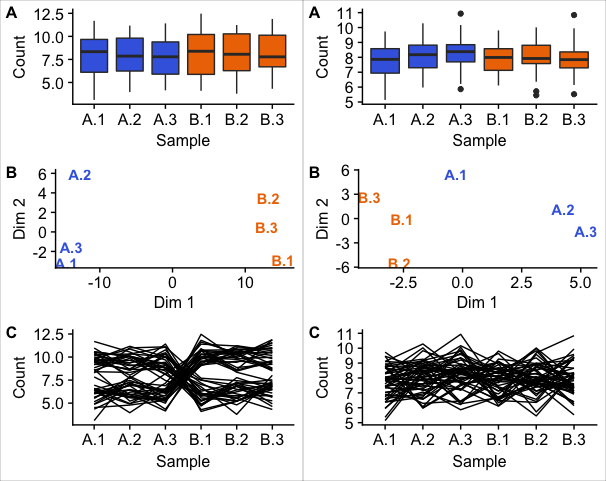
\includegraphics[width=15cm]{/Users/lindz/JDSPaper/Bioinformatics/Pictures/bmp/Color/2group.png}}}
\end{center}
\caption{Caption.
\label{2group}}
\end{figure}

\section{Scatterplot matrices}
\label{s:Scatterplot matrices}

Pairwise scatterplot matrices are another effective multivariate visualization tool that plot the mapped read count distributions across all genes and samples. A scatterplot matrix draws each row (gene) in the data table as a point in each scatterplot. With these plots, users can quickly discover unexpected patterns, recognize geometric shapes, and assess the structure and association between multiple variables simultaneously. 

The ideal dataset will have larger variability between treatment groups than between replicates. As Figure~\ref{cotyIdeal} shows, researchers can quickly confirm this with a scatterplot matrix. Within each scatterplot, most genes should fall along the \textit{x=y} line (in red) as we expect only a small proportion of genes to show differential expression between samples. However, if the data has lower variability between replicates than between treatments, then we expect the spread of the scatterplot observations to fall more closely along the \textit{x=y} relationship between replicates than between treatments. Indeed, in Figure~\ref{cotyIdeal}, we created a scatterplot matrix for a public RNA-seq dataset that contains three replicates for two developmental stages of soybean cotyledon (S1 and S2). We can immediately verify that the nine scatterplots between treatments (in the bottom-left corner of the matrix) have more spread around the \textit{x=y} line than the six scatterplots between replicates.

\begin{figure}
\begin{center}
\centerline{\fbox{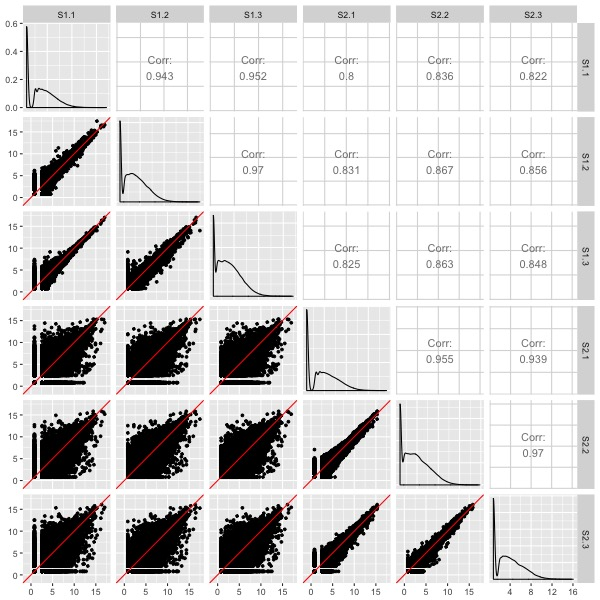
\includegraphics[width=15cm]{/Users/lindz/JDSPaper/Bioinformatics/Pictures/SwitchSample/Switch12/NotSwitch/S1_S2_points_size1.jpg}}}
\end{center}
\caption{Caption.
\label{cotyIdeal}}
\end{figure}

After confirming this expected trend, users can also use the scatterplot matrix to focus on subsets of genes: Outlier genes that deviate from the \textit{x=y} line in replicate scatterplots are problematic genes, whereas outlier genes that deviate from the \textit{x=y} line in treatment scatterplots are potential differentially expressed genes. In order to achieve this capability, users must be able to interact with the plot. Figure # shows a static screenshot of this capability, but the interactive version of this plot is available at #.

Notice that our scatterplot matrix contains 15 scatterplots and that each gene is denoted as a point in all scatterplots. With 73,320 genes in our data, more than one million points must be plotted. Rendering all points interactive can significantly slow down the interactive capabilities of the plot. To solve this, as shown in Figure #, we can tailor the geometric object of the scatterplots to be hexagon bins rather than points. This dramatically reduces the number of objects to be plotted, which increases the interactivity speed.

The interactive version of the plot demonstrates that the user can determine the number of genes in a particular hexagon bin by hovering over it. By clicking on a particular hexagon bin, the genes contained in that hexagon bin are superimposed as orange points across all scatterplots. 


"Glyma06g11430.1" "Glyma13g02510.1" S1.2 high (S1 low, S2 high) (click on S1.1 and S1.2)

\begin{table}
\caption{This is a simple table.}
\label{t:one}
\begin{center}
\begin{tabular}{lrrr}
\Hline
Culture/Library prep. & \multicolumn{1}{c}{Library prep. protocol} &  \multicolumn{1}{c}{Growth condition} & \multicolumn{1}{c}{Flow-cell} \\ \hline
Y1 & Protocol 1 & YPD & 428R1 \\
Y1 & Protocol 1 & YPD & 4328B \\
Y2 & Protocol 1 & YPD & 428R1 \\
Y2 & Protocol 1 & YPD & 4328B \\
Y7 & Protocol 1 & YPD & 428R1 \\
Y7 & Protocol 1 & YPD & 4328B \\
Y4 & Protocol 2 & YPD & 61MKN \\
Y4 & Protocol 2 & YPD & 61MKN \\
\hline
\end{tabular}
\end{center}
\end{table}

You can experiment with fancier tables than Table~\ref{t:one}.

We can get bold symbols using \verb+\bmath+, for example, $\bmath{\alpha}_i$.

\section{Discussion}
\label{s:discuss}

Put your final comments here. 

%  The \backmatter command formats the subsequent headings so that they
%  are in the journal style.  Please keep this command in your document
%  in this position, right after the final section of the main part of 
%  the paper and right before the Acknowledgements, Supplementary Materials,
%  and References sections. 

\backmatter

%  This section is optional.  Here is where you will want to cite
%  grants, people who helped with the paper, etc.  But keep it short!

\section*{Acknowledgements}

The authors thank Professor A. Sen for some helpful suggestions,
Dr C. R. Rangarajan for a critical reading of the original version of the
paper, and an anonymous referee for very useful comments that improved
the presentation of the paper.\vspace*{-8pt}

%  If your paper refers to supplementary web material, then you MUST
%  include this section!!  See Instructions for Authors at the journal
%  website http://www.biometrics.tibs.org

\section*{Supplementary Materials}


%  Here, we create the bibliographic entries manually, following the
%  journal style.  If you use this method or use natbib, PLEASE PAY
%  CAREFUL ATTENTION TO THE BIBLIOGRAPHIC STYLE IN A RECENT ISSUE OF
%  THE JOURNAL AND FOLLOW IT!  Failure to follow stylistic conventions
%  just lengthens the time spend copyediting your paper and hence its
%  position in the publication queue should it be accepted.

%  We greatly prefer that you incorporate the references for your
%  article into the body of the article as we have done here 
%  (you can use natbib or not as you choose) than use BiBTeX,
%  so that your article is self-contained in one file.
%  If you do use BiBTeX, please use the .bst file that comes with 
%  the distribution.  In this case, replace the thebibliography
%  environment below by 
%
%  \bibliographystyle{biom} 
% \bibliography{mybibilo.bib}

\begin{thebibliography}{}

\bibitem{ } Anders, S. and Huber, W. (2010). Differential expression analysis for sequence count data. \textit{Genome Biology} \textbf{11,} R106.

\bibitem{ } Anders, S., Reyes, A., and Huber, W. (2012). Detecting differential usage of exons from RNA-seq data. \textit{Genome Research} \textbf{22,} 2008–2017.

\bibitem{ } Bullard, J. H., Purdom, E., Hansen, K. D., and Dudoit, S. (2010). Evaluation of statistical methods for normalization and differential expression in mRNA-Seq experiments. \textit{BMC Bioinformatics} \textbf{11,} 94.

\bibitem{ } Grabherr, M. G., Haas, B. J., Yassour, M., Levin, J. Z., Thompson, D. A., Amit, I., et al. (2011). Full-length transcriptome assembly from RNA-Seq data without a reference genome. \textit{Nature Biotechnology} \textbf{29,} 644–652.

\bibitem{ } Hansen, K.D., Brenner, S.E., and Dudoit, S. (2010). Biases in Illumina transcriptome sequencing caused by random hexamer priming. \textit{Nucleic Acids Research} \textbf{38,} e131.

\bibitem{ } Huber, W., Carey, V.J., Gentleman, R,, Anders, S,, Carlson, M., and Carvalho, B.S. (2015). Orchestrating high-throughput genomic analysis with Bioconductor. \textit{Nature Methods} \textbf{12,} 115-121.

\bibitem{ } Law, C.W., Chen, Y., Shi, W., and Smyth, G.K. (2014). voom: precision weights unlock linear model analysis tools for RNA-seq read counts. \textit{Genome Biology} \textbf{15,} R29.

\bibitem{ } Love, M.I., Huber, W., and Anders, S. (2014). Moderated estimation of fold change and dispersion for RNA-seq data with DESeq2. \textit{Genome Biology} \textbf{15,} 550.

\bibitem{ } Marini, F. (2017). pcaExplorer: Interactive Visualization of RNA-seq Data Using a Principal Components Approach. GitHub, Inc. https://github.com/federicomarini/pcaExplorer (accessed October 7, 2017).

\bibitem{ } Marioni, J.C., Mason, C.E., Mane, S.M., Stephens, M., and Gilad, Y. (2008). RNA-seq: an assessment of technical reproducibility and comparison with gene expression arrays. \textit{Genome Research} \textbf{18,} 1509–1517.

\bibitem{ } McIntyre, L.M., Lopiano, K.K., Morse, A.M., Amin, V., Oberg, A.L., Young, L.J., et al. (2011). RNAseq: technical variability and sampling. \textit{BMC Genomics} \textbf{12,} 293.

\bibitem{ } Morin, R., Bainbridge, M., Fejes, A., Hirst, M., Krzywinski, M., Pugh, T., et al. (2008). Profiling the HeLa S3 transcriptome using randomly primed cDNA and massively parallel short-read sequencing. \textit{Biotechniques} \textbf{45,} 81–94.

\bibitem{ } Oshlack, A., Robinson, M.D., and Young, M.D. (2010). From RNA-seq reads to differential expression results. \textit{Genome Biology} \textbf{11,} 220.

\bibitem{ } Pan, Q., Shai, O., Lee, L. J., Frey, B. J., and Blencowe, B. J. (2008). Deep surveying of alternative splicing complexity in the human transcriptome by high-throughput sequencing. \textit{Nature Genetics} \textbf{40,} 1413–1415.

\bibitem{ } Risso, D., Schwartz, K., Sherlock, G., Dudoit, S. (2011). GC-Content Normalization for RNA-Seq Data. \textit{BMC Bioinformatics} \textbf{12,} 480.

\bibitem{ } Ritchie, M.E., Phipson, B., Wu, D., Hu, Y., Law, C.W., Shi, W., and Smyth, G.K. (2015). limma powers differential expression analyses for RNA-sequencing and microarray studies. \textit{Nucleic Acids Research} \textbf{43,} e47.

\bibitem{ } Robertson, G., Schein, J., Chiu, R., Corbett, R., Field, M., Jackman, S. D., et al. (2010). De novo assembly and analysis of RNA-seq data. \textit{Nature Methods} \textbf{7,} 909–912.

\bibitem{ } Robinson, M.D. and Oshlack, A. (2010). A scaling normalization method for differential expression analysis of RNA-seq data. \textit{Genome Biology} \textbf{11,} R25.

\bibitem{ } Robinson, M.D., McCarthy, D.J., and Smyth, G.K. (2010). edgeR: a Bioconductor package for differential expression analysis of digital gene expression data. \textit{Bioinformatics} \textbf{26,} 139–140.

\bibitem{ } Shneiderman, B. (2002). Inventing Discovery Tools: Combining Information Visualization with Data Mining. \textit{Information Visualization} \textbf{1,} 5-12.

\bibitem{ } Schurch, N.J., Schofield, P., Gierliński, M., Cole, C., Sherstnev, A., Singh, V., et al. (2016). How many biological replicates are needed in an RNA-seq experiment and which differential expression tool should you use? \textit{RNA} \textbf{22,} 839–851.

\bibitem{ } Shu, S., Ritchie, M.E., Law, C., and Lee, S. (2016). Glimma: Interactive HTML graphics. GitHub, Inc. https://github.com/Shians/Glimma/ (accessed October 7, 2017).

\bibitem{ } Trapnell, C., Hendrickson, D.G., Sauvageau, M., Goff, L., Rinn, J.L., and Pachter, L. (2013). Differential analysis of gene regulation at transcript resolution with RNA-seq. \textit{Nature Biotechnology} \textbf{31,} 46–53.

\bibitem{ } Trapnell, C., Roberts, A., Goff, L., Pertea, G., Kim, D., and Kelley D.R. (2012). Differential gene and transcript expression analysis of RNA-seq experiments with TopHat and Cufflinks. \textit{Nature Protocols} \textbf{7,} 562–578.

\bibitem{ } Unwin, A. (1992). How interactive graphics will revolutionize statistical practice. \textit{The Statistician} \textbf{41,} 365-369

\bibitem{ } Wang, Z., Gerstein, M., and Snyder, M. (2009). RNA-Seq: a revolutionary tool for transcriptomics. \textit{Nature Reviews Genetics} \textbf{10,} 57–63.

\bibitem{ } Zhao, S., Fung-Leung, W.-P., Bittner, A., Ngo, K., and Liu, X. (2014). Comparison of RNA-Seq and Microarray in Transcriptome Profiling of Activated T Cells. \textit{PLoS ONE} \textbf{9,} e78644.





\end{thebibliography}

\appendix

%  To get the journal style of heading for an appendix, mimic the following.

\section{}
\subsection{Title of appendix}

Put your short appendix here.  Remember, longer appendices are
possible when presented as Supplementary Web Material.  Please 
review and follow the journal policy for this material, available
under Instructions for Authors at \texttt{http://www.biometrics.tibs.org}.

\label{lastpage}

\end{document}
